\documentclass[10pt]{beamer}
\usepackage{bbm}
\usepackage{fontspec}

\usepackage{graphicx}
\usepackage{animate}
\renewcommand\appendixname{Appendix}
\usepackage{xcolor}
\usepackage{tikz}
\colorlet{rred}{red!80!black}
\colorlet{ggreen}{green!80!black}




\usetheme[progressbar=foot]{metropolis}
\usepackage{appendixnumberbeamer}
\setbeamercovered{dynamic}

\usepackage{booktabs}
\usepackage[scale=2]{ccicons}

\usepackage{pgfplots}
\usepgfplotslibrary{dateplot}
\setbeamertemplate{caption}{\raggedright\insertcaption\par}
\setlength{\abovecaptionskip}{-10pt plus 0pt minus 0pt}

\usepackage{xspace}
\newcommand{\themename}{\textbf{\textsc{metropolis}}\xspace}
\theoremstyle{definition}
\newtheorem{defn}{Definition}
\newtheorem{obs}{Observation}

% math symbols
\newcommand{\R}{\mathbb{R}}
\newcommand{\N}{\mathbb{N}}
\newcommand{\Z}{\mathbb{Z}}
\newcommand{\E}{\mathbb{E}}
\newcommand{\1}{\mathbbm{1}}
\newcommand{\XX}{\mathcal{X}}
\newcommand{\TT}{\mathcal{T}}
\newcommand{\YY}{\mathcal{Y}}
\newcommand{\UU}{\mathcal{U}}
\newcommand{\VV}{\mathcal{V}}
\newcommand{\WW}{\mathcal{W}}
\newcommand{\LL}{\mathcal{L}}

\DeclareMathOperator*{\argmin}{argmin}
\DeclareMathOperator*{\argmax}{argmax}
\title{An introduction to PCA}
\subtitle{Weekly AI pills}
\date{2020-10-16}
\author{Fabio Brau.}
\institute{SSSA, Emerging Digital Technologies, Pisa.}
% \titlegraphic{\hfill\includegraphics[height=1.5cm]{logo.pdf}}

\usebackgroundtemplate{%
    \begin{picture}(300,271)
      \hspace{11.2cm}
       
\includegraphics[scale=0.1]{pic/logoretis_noname.png}
   \end{picture}}

\begin{document}
{\usebackgroundtemplate{%
    \begin{picture}(300,265)
      \hspace{0.9cm}
       
\includegraphics[scale=0.5]{pic/tecip_logo.png}
       \hspace{0.5cm}
       
\includegraphics[scale=0.21]{pic/logoretis_320.png}
   \end{picture}}%
\maketitle
}
\begin{frame}{Summary}
  \begin{itemize}
    \item Geometrical Introduction
    \item Classical Derivation
    \item Dimensionality Reduction
    \item Statistical Point of View
    \item Non Linear PCA
  \end{itemize}
\end{frame}
\begin{frame}{Introduction: Principal Component Analysis}{}
    {\it ``The aim of Principal Component Analysis is to reduce the
    dimensionality of a dataset without loosing the relations between variables.''}
  \begin{enumerate}
    \item {\bf Pearson} (1901) Introduced PCA by focusing on geometric
      optimization problem.\\
      He stated that his method ``can be easily applied
      to numerical problem'' but the calculation becomes ``cumbersome'' for
      more than $4$ variables.
    \onslide<2->
    \item {\bf Hotelling} (1933) Introduced PCA by focusing on {\bf Factor
      Analysis}.\\
      He introduced the term {\bf Principal Component}
  \end{enumerate}
\end{frame}
\section{Geometrical Introduction}
\begin{frame}{Geometrical Introduction}
  Let $X \in \R^{N\times n}$ be a dataset of $N$
  {\bf observation} within $n$ {\bf variables}. 
  \begin{equation}
    X =
    \begin{bmatrix}
      \, & x_1 ^ T &\,\\
      \, & \vdots &\,\\
      \, & x_N ^ T &\,\\
    \end{bmatrix}
    =
    \begin{bmatrix}
      & & & \\
      x^{(1)} &\vline& \cdots& \vline& x^{(n)}\\
      & & & \\
    \end{bmatrix}
    \label{Geometrical view}
  \end{equation}
  {\bf Notations:}
  \begin{itemize}
    \item $x_i\in\R^n$ represents a single {\bf observation}, i.e a {\bf
      sample} in the feature space.
    \item $x^{(i)}\in\R^N$ represents the single {\bf variable}, i.e a {\bf
      column} of the dataset.
    \item $X$ is centered if $X^T\1_N=0$, where $\1_n=[1,\cdots,1]^T$.
  \end{itemize}
\end{frame}
\begin{frame}{Geometrical Introduction: Finding a principal direction.}
  \begin{minipage}{0.5\textwidth}
    \begin{enumerate}
      \item \uncover<1->{Scalar product measures the projection of $x_j$ along
        the direction $w$.}
      \item \uncover<2->{We are only interested on module.}
      \item \uncover<3->{Summation over samples to get the global
        projection's contribute.}
      \item \uncover<4->{Searching for $w$ which maximizes projection.}
      \item \uncover<5->{Adding constraint to avoid $w\to\infty$ solution.}
    \end{enumerate}
  \end{minipage}\hfill
  \begin{minipage}{0.4\textwidth}
      \begin{equation*}
        \uncover<4->{w_1 \in\argmax_{\uncover<5>{\|w\|_2 = 1}}}
        \uncover<3->{\sum_{j=1}^N}
        \uncover<2->{\left(}\uncover<1->{w\cdot x_j}\uncover<2->{\right)^2}
      \end{equation*}
    \begin{figure}[b]
      \centering
      \includegraphics<1-2>[clip, scale=0.3, trim=3.1cm 0 0cm 0cm]{./pic/dummy_2.eps}
      \includegraphics<3->[clip, scale=0.3, trim=3.1cm 0 0cm 0cm]{./pic/dummy_3.eps}
    \end{figure}
  \end{minipage}
\end{frame}
\begin{frame}{Geometrical Introduction: Finding other directions}
  We search for other orthogonal directions which maximize projections.
  \begin{equation*}
  \begin{aligned}
    w_1 \in \argmax_{\|w\|_2=1}\sum_{j=1}^N (w\cdot x)^2 &\\
    w_2 \in \argmax_{\|w\|_2=1}\sum_{j=1}^N (w\cdot x)^2 &\quad\mbox{and}\quad w_2\perp w_1\\
    \vdots \\
    w_n \in \argmax_{\|w\|_2=1}\sum_{j=1}^N (w\cdot x)^2
    &\quad\mbox{and}\quad w_n\perp \left\{
    w_1,\ldots,w_{n-1} \right\}
  \end{aligned}
\end{equation*}
\begin{center}
  \href{./pic/PCA_3D.html}{\bf Example}
\end{center}
\end{frame}
\metroset{block=fill}
\begin{frame}{Geometrical Introduction: Direction Selection}
  \[
    V(w)=\sum_j (w \cdot x_j)^2 \qquad\mbox{\bf momentum along $w$}
  \]
  \onslide<2->
  If $w_1,\,w_2,\,w_3$ orthogonal that maximizes $V$ in the 3D example, then
  \begin{enumerate}
    \item $V(w_1) =  3181.20$\hfill\uncover<3->{\approx82.5\%}
    \item $V(w_2) = 646.25$\hfill\uncover<3->{\approx 17.0\%}
    \item $V(w_3) = 19.23$ \hfill\uncover<3->{\approx 0.5 \%}
  \end{enumerate}
    \onslide<4->
    \begin{center}
      {\bf What if we forget the last direction?}
    \end{center}
  \onslide<5->
  \begin{block}{Observation}
    \begin{itemize}
        \item $x_j =\alpha_{1j}w_1+\alpha_{2j}w_2+\alpha_{3j}w_3$
          (where $\alpha_{ij} = w_i\cdot x_j$).
        \item $\tilde x_j = \alpha_{1j}w_1 + \alpha_{2j}w_2$. 
    \end{itemize}
    \begin{equation}
      \frac{1}{N}\sum_j \|x_j - \tilde x_j\|^2 = \frac{V(w_3)}{N}\approx
      4.8\,10^{-3}
      \tag{MSE}
    \end{equation}
  \end{block}
\end{frame}
\begin{frame}{Geometrical Introduction: Conclusion}
  \begin{itemize}
    \item Given a set of data $X\in\R^{N\times n}$
    \item We can find $w_1,\cdots,w_n$ principal (orthonormal) directions the
      maximize their momentum.
    \item $V(w_1) > V(w_2)>\cdots> V(w_n)$
    \item Approximating X with $\tilde X$ by taking only the first $k$
      directions we are getting an error that depends on $V(w_i)$.
  \end{itemize}
  \onslide<2->
  {\bf\centering What's the catch?}
  \onslide<3->
   \begin{equation}
     \begin{aligned}
       \max_{w\in\R^n}\quad & \sum_{j=1}^N (w \cdot x_j)^2\\
       \mbox{s.t}\quad & w_i \cdot w =0, \,\forall i<k \\
       & w\cdot w = 1\\
    \end{aligned}
    \label{MP}
    \tag{MP}
  \end{equation} 
\end{frame}
\section{Classical Derivation}
\begin{frame}{Classical Derivation: An Eigenvalue Problem}
  \[
    \max_{\|w\|=1} V(w) =\max_{\|w\|=1} \sum_j (w^Tx_j)^2 = \max_{w^Tw=1}
    w^T(X^TX)w  
    \tag{MP}
  \]
  \onslide<2->
  \begin{center}
    {\bf Lagrange Multipliers Technique}
  \end{center}
  Let consider the Lagrangian Function of \ref{MP}
  \[
    \LL(w,\lambda) = V(w) - \lambda(w^Tw -1),\quad\forall w
    \in\R^n,\,\lambda\in\R
  \]
  \begin{block}{Claim}
  If $w^*$ is a solution of \ref{MP} then there exists $\lambda^*$ such that
  \begin{equation}
    \nabla \LL(w^*,\lambda^*)=0,\quad i.e\quad
      (X^TX) w^* -\lambda^*w^*=0
  \end{equation}
  \end{block}
  \onslide<3->
  \[
    w\, \mbox{\bf Principal Direction}\quad\iff\quad w\,
    \mbox{\bf Eigenvector of}\, X^TX
  \]
\end{frame}
\begin{frame}{Classical Derivation: An Eigenvalue Problem}
  \begin{center}
    {\bf Why switching to an eigen-pair
    problem?}\footnote{Appendix for further details.}
  \end{center}
  \onslide<2->
  \begin{minipage}[t]{0.5\textwidth}
    \begin{minipage}[t]{0.3\textwidth}
      \vfill
      $X^TX\qquad +\qquad$
    \end{minipage}
    \begin{minipage}[t]{0.3\textwidth}
      \begin{figure}[h!]
        \centering
        \includegraphics<2->[scale=0.10, trim=0cm 0cm 0 3cm]{./pic/matlab.png}
      \end{figure}
    \end{minipage}
    \begin{minipage}[t]{0.1\textwidth}
    \vfill
    $\qquad\longrightarrow$
    \end{minipage}
  \end{minipage}\hfill
  \begin{minipage}[t]{0.5\textwidth}
    \vspace{-0.4cm}
    \begin{itemize}
      \item $w_1,\cdots,w_n$ \hfill {\bf eigenvectors}
      \item $w_i^TX^TXw_i=V(w_i)$ \hfill{\bf eigenvalues}
      \item $V(w_1)>\cdots>V(w_n)\ge 0$
    \end{itemize}
  \end{minipage}
\end{frame}
\section{Dimensionality Reduction}
\begin{frame}{Dimensionality Reduction}
  The matrix $W=[w_1|\cdots|w_n]$ can be used to reduce the dimensionality
  \[
    F=
    \begin{bmatrix}
      f^{(1)}&|\cdots|&f^{(n)}
    \end{bmatrix}
    = X\,W\quad\mbox{\bf (factors scores)}
  \]
  \begin{minipage}[t]{0.4\textwidth}
    \begin{figure}[h!]
      \centering
      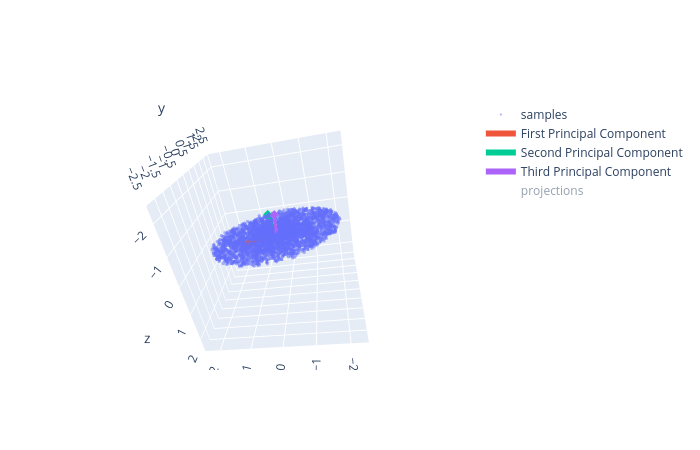
\includegraphics[clip, scale=0.4, trim=1cm 1.5cm 8cm 4cm]{./pic/PCA_3D.png}
      \caption{Feature space}
    \end{figure}
  \end{minipage}\hfill
  \begin{minipage}[t]{0.5\textwidth}
    \begin{figure}[h!]
      \centering
      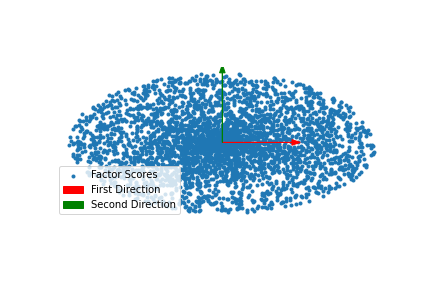
\includegraphics[scale=0.3]{./pic/PCA_2D.png}
      \caption{Factor scores restricted to the first two principal
      directions.}
    \end{figure}
  \end{minipage}
\end{frame}
\begin{frame}{Dimensionality Reduction: A concrete example}{}
  \begin{minipage}[t]{0.5\textwidth}
    \begin{figure}[h!]
      \centering
      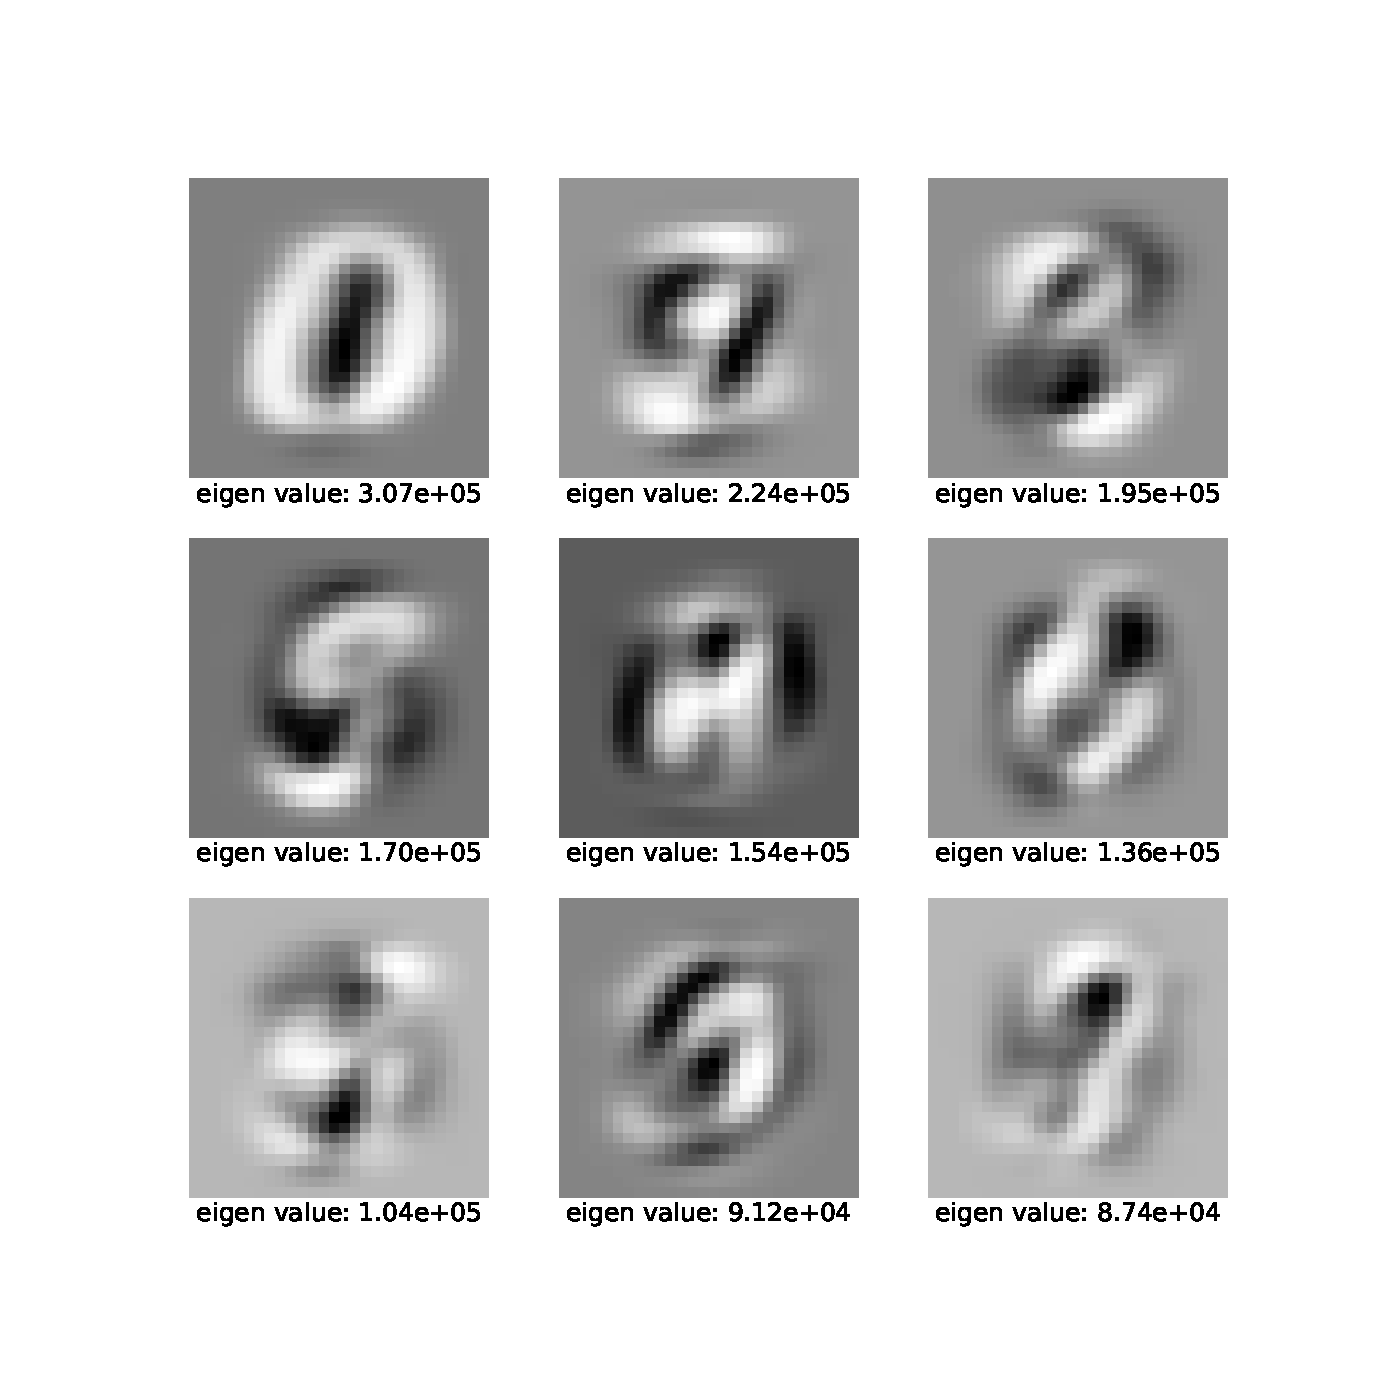
\includegraphics[scale=0.28, trim=0 0 0 5cm]{./pic/eigen_digits.eps}
   \end{figure}
  \end{minipage}\hfill
  \begin{minipage}[t]{0.4\textwidth}
  {\bf MNIST}: hand-written digits expressed as $28\times28$ images of
  $8$-bit.\\ 
  $\\$
  {\bf Samples:} $60k$\\
  {\bf Variables:} $784$\\
  {\bf Range:} $0-255$
  \end{minipage}\\
  First 9 Eigen-Digits, i.e eigen vectors of $X^TX$.
\end{frame}
\begin{frame}{Dimensionality Reduction: A concrete example}
  %\animategraphics[loop,controls,width=0.5\linewidth]{2}{./pic/mnist/compress-}{0}{15}
  \begin{minipage}[t]{0.4\textwidth}
    \begin{figure}[h!]
      \centering
      \includegraphics<1>[scale=0.3]{./pic/mnist/compress-1.eps}%
      \includegraphics<2>[scale=0.3]{./pic/mnist/compress-10.eps}%
      \includegraphics<3>[scale=0.3]{./pic/mnist/compress-20.eps}%
      \includegraphics<4>[scale=0.3]{./pic/mnist/compress-100.eps}%
      \includegraphics<5>[scale=0.3]{./pic/mnist/compress-200.eps}%
      \includegraphics<6>[scale=0.3]{./pic/mnist/compress-500.eps}%
      \includegraphics<7->[scale=0.3]{./pic/mnist/compress-700.eps}%
    \end{figure}
  \end{minipage}\hfill
  \begin{minipage}[t]{0.5\textwidth}
    \begin{figure}[h!]
      \centering
      \includegraphics<1>[scale=0.3]{./pic/mnist/cum_eig-1.eps}%
      \includegraphics<2>[scale=0.3]{./pic/mnist/cum_eig-10.eps}%
      \includegraphics<3>[scale=0.3]{./pic/mnist/cum_eig-20.eps}%
      \includegraphics<4>[scale=0.3]{./pic/mnist/cum_eig-100.eps}%
      \includegraphics<5>[scale=0.3]{./pic/mnist/cum_eig-200.eps}%
      \includegraphics<6>[scale=0.3]{./pic/mnist/cum_eig-500.eps}%
      \includegraphics<7->[scale=0.3]{./pic/mnist/cum_eig-700.eps}%
    \end{figure}
  \end{minipage}
  \begin{block}{Compression Error Estimation}{}
    \begin{enumerate}
      \item $x\in\R^{n}$ original sample.
      \item $f = W^T x\in\R^{n}$ coordinates in factor-scores space.
      \item $\tilde f = [f_1,\cdots,f_{k}]\in\R^{n-k}$ taking first $k$ coordinates.
    \item $\tilde x = [w_1|\cdots|w_{k}]\, \tilde f\in\R^{n}$, approximation of $x$.
    \end{enumerate}
    \onslide<8->
    \[
      \|x-\tilde x\|\approx\sqrt{\frac{1}{N}\sum_j\| x_j - \tilde x_j\|^2}= 
      \frac{1}{\sqrt{N}}\sqrt{V(k+1)+\cdots+V(n)}
      \label{ErrorBound}
      \tag{EB}
    \]
  \end{block}
\end{frame}
\section{Where is statistic?}
\begin{frame}{Statistical Point of View: Notations}{}
$\VV$ random variable, $V = (v_1,\ldots,v_N)$ N observations of the variable. 
  \begin{itemize}
    \item\uncover<2->{{\bf Expected Value} \hfill $\E[\VV] =
      \frac{1}{N}\sum_{j=1}^N v_j$} 
    \item\uncover<3->{{\bf Variance} \hfill $Var(\VV) = \E[(\VV -
      \E[\VV])^2]$}
    \item\uncover<4->{{\bf Covariance} \hfill $Cov(\UU,\VV) = \E[(\UU -
      \E[\UU])(\VV - \E[\VV])]$}
  \item\uncover<5->{If $\UU = (\UU_1,\cdots,\UU_m)$, then 
      \[
        Cov(\UU)=
        \begin{bmatrix}
          Cov(\UU_1,\UU_1) & \cdots & Cov(\UU_1,\UU_m)\\
          \vdots & \ddots & \vdots \\
          Cov(\UU_m,\UU_1)& \cdots & Cov(\UU_m,\UU_m)
        \end{bmatrix}
      \]}
  \end{itemize}
  \onslide<6->

  {\bf Observations}\\
  Under the assumption $\E[\UU]=\E[\VV]=0$
  \begin{enumerate}
    \item $Var(\VV)=\frac{1}{N}\sum_{j=1}^N v_j^2$
    \item $Cov(\UU,\VV) = \frac{1}{N}\sum_{j=1}^N u_jv_j$ 
    \item If $\UU = (\UU_1,\cdots,\UU_m)$, then 
      \[
        \mbox{Var}(w\cdot \UU) = w^T\mbox{Cov}(\UU) w
      \]
  \end{enumerate}
\end{frame}
\begin{frame}{Statistical Point of View: Language Translation}
  \begin{minipage}[t]{0.4\textwidth}
    \begin{center}
      {\bf Geometrical}
    \end{center}
    \begin{itemize}
      \item\uncover<2->{$X^T\1_N = 0$}
      \item\uncover<3->{eig of $X^TX$}
      \item\uncover<4->{$V(w) = \sum_j (w\cdot x_j)^2$ momentum along $w$.}
    \end{itemize}
  \end{minipage}\hfill
  \begin{minipage}[t]{0.4\textwidth}
    \begin{center}
      {\bf Statistical}
    \end{center}
    \begin{itemize}
      \item\uncover<2->{$\E[X^{(1)}], \cdots, \E[X^{(n)}]=0$.}
      \item\uncover<3->{eig of $N\,\mbox{Cov}(X)$}
      \item\uncover<4->{$N\,\mbox{Var}(w\cdot X)$}
    \end{itemize}
  \end{minipage}
  \begin{figure}[!h]
    \centering
    \includegraphics<5>[trim=0 4cm 0 0 0]{./pic/spider_man.png}
  \end{figure}
  \vspace{-1cm}
  \visible<6->{%
  \begin{minipage}[t]{\textwidth}
    \begin{block}{Compression Error Estimation}
    \begin{equation*}
      \|x_j -\tilde x_j\|\approx \sqrt{\E[\|x_j -\tilde x_j\|^2]}=
        \sqrt{Var(w_{k+1}\cdot X) +\cdots+ Var(w_n\cdot X)}
    \end{equation*} 
    a.k.a
    \[
      w_1,\cdots,w_{k} \quad\mbox{explain}\quad 100*\left(\frac{\sum_{i=1}^k
      \mbox{Var}(w_i\cdot X)}{\sum_i \mbox{Var}(w_i\cdot X)}\right)\, \%\quad
      \mbox{of the variance.}
    \]
    \end{block}
  \end{minipage}}
\end{frame}
\section{Non Linear PCA}
\begin{frame}{Non Linear PCA: Kernel PCA}
  \begin{minipage}[t]{0.4\textwidth}
    \begin{equation*}
      \begin{aligned}
        V_{\kappa}(w) = &\sum_j \kappa(w, x_j)^2\\
        &\mbox{where} \\
        \kappa(v,w)= & \Phi(v)\cdot\Phi(w)
      \end{aligned}
    \end{equation*}
  \end{minipage}\hfill
  \begin{minipage}[t]{0.4\textwidth}
    \begin{figure}[h!]
      \centering
      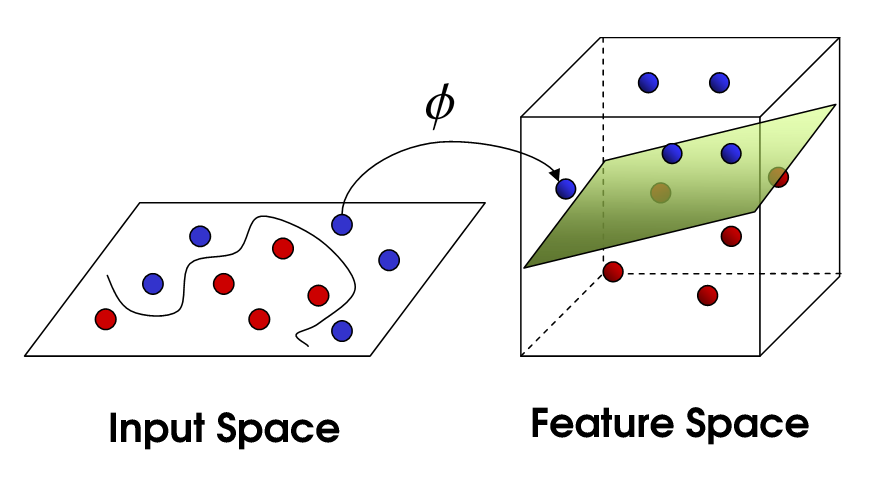
\includegraphics[scale=0.15]{./pic/kernel-trick.png}
    \end{figure}
  \end{minipage}\vfill
  \onslide<2->
  \href{https://ieeexplore.ieee.org/servlet/opac?bknumber=6267332}%
  {\bf Learning with kernels - Bernhard Schölkopf, Alexander J. Smola}

\end{frame}
\begin{frame}{Non Linear PCA: Autoencoders}
  \begin{minipage}[t]{0.5\textwidth}
      \begin{figure}[h!]
      \centering
      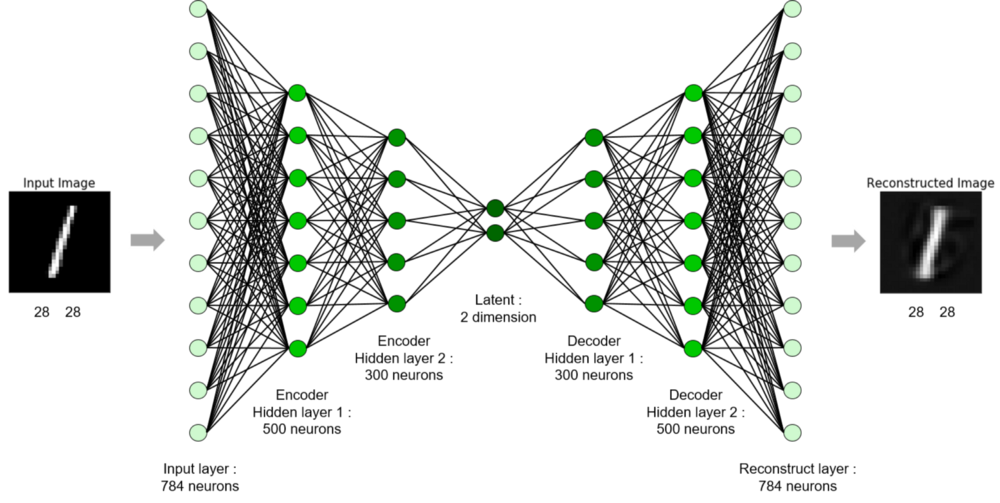
\includegraphics[scale=0.15, trim=0 0 0 5cm]{./pic/enc-dec.png}
    \end{figure}
  \end{minipage}%
  \begin{minipage}[t]{0.5\textwidth}
    \begin{center}
      {\bf Autoencoders Training}
    \end{center}
    \begin{equation}
      \min_\theta \frac{1}{N}\sum_{j} \|f_\theta(x_j) - x_j\|^2
      \label{autotrain}
      \tag{mP}
    \end{equation}
  \end{minipage}
  \vfill
\onslide<2-> 
\begin{block}{Claim\footnote{\href{https://arxiv.org/pdf/1804.10253.pdf}{\bf
      From Principal Subspaces to Principal Components with Linear
Autoencoders}}}
  \begin{itemize}
    \item $f_\theta(x)= U\,V\,x$ is a 1-depth autoencoder with hidden space of
    dimension $k$.
  \item If $W=[w_1|\cdots|w_n]$ principal components of $X\in\R^{N\times n}$
  \item $V^*= [w_1|\cdots|w_k]$ and $U^*=(V^*)^T$ solves~\ref{autotrain}
  \end{itemize}
\end{block}
\end{frame}
\begin{frame}
  \begin{center}
    {\bf Thanks for the attention.}
  \end{center}
\end{frame}
\appendix
\section{appendix}
\begin{frame}{Eigen-pairs of Simmetric def.positive matrices}
  A matrix $A\in M(n)$ is symmetric and def.positive if respectively 
  \begin{equation}
    A^TA=AA^T,\quad v^TAv > 0\,\forall v\in\R^n
  \end{equation}
  From spectral theorem it's exists an isometry $V=[v_1|\cdots|v_n]$ such
  that 
  \[
    V^TAV = D
  \]
  where $D=\mbox{diag}(\lambda_1,\cdots,\lambda_n)$ is a diagonal matrix.\\
  Because of $V^TV=Id$ then 
  \begin{equation}
    AV =
    \begin{bmatrix}
      Av_1&|\cdots|&Av_n
    \end{bmatrix}= VD =
    \begin{bmatrix}
      \lambda_1v_1&|\cdots|&\lambda_nv_n
    \end{bmatrix}
  \end{equation}
  This shows that {\bf there exists an orthonormal bases of eigenvectors for
  $A$}.
  Because of $A$ is def.positive then 
  \[
    \lambda_i = v_i^TAv_i >  0
  \]
  and so {\bf $A$ has only positive eigenvalues}.
\end{frame}
\begin{frame}{Approximation Error}
  For each $j=1,\cdots,N$ we can write $x_j = f_{j1}v_i+\cdots+f_{jn}v_n$
  where $f_{ij} = w_i\cdot x_j$. The approximated samples can be written as
  $\tilde x_j = f_{j1}v_i+\cdots+f_{j,n-k}v_{n-k}$. The main idea is to write
  the {\bf expected value of the square euclidean distance} between the two
  samples (i.e. original end compressed).
  \begin{equation}
    \begin{aligned}
      \|x - \tilde x\|^2&\approx \frac{1}{N} \sum_{j=1}^N
      \|f_{j,n-k+1}v_{n-k+1} + \cdots + f_nv_n\|^2 \\
      &=\frac{1}{N}\sum_{j=1}^N f_{j,n-k+1}^2+\cdots+f_{j,n}^2\\
      &=\frac{1}{N}\left(V(w_1)+\cdots+V(w_n)\right)
    \end{aligned}
  \end{equation}
  By taking the root we obtain the approximation in~\ref{ErrorBound}.
  Moreover we can compute also the {\bf Variance of the squared euclidean
  distance} to increase the accuracy of the error approximation.
\end{frame}
\end{document}

